\chapter{Korrespondance Analyse} \label{sec:Kor}
Korrespondance problemet, imellem to eller flere billeder af samme objekt, referere til problemet om at finde et sæt af punkter i det ene billede, der kan identificeres og matches i det andet.
Udfordringen ved problemet ligger i at billederne, der skal matches, er udsat for en række ændringer, det kan f.eks. være forskydning i kameraets position ift. scenen eller  ændringer i scenens motiv. Et godt eksempel på korrespondance problemet er det menneskelige syn. Øjnene agere som to kameraer, der hver især fanger deres billede og omdanner disse billeder til ét sammenhængende panoramisk billede, ved hjælp af oprettelse af korrespondancer. Korrespondancen mellem øjnene tillader også opfattelse af dybde i billedet, hvilket skyldes den horisontale forskydning af menneskets øjne. Denne sektion vil beskrive, hvordan denne korrespondance kan efterlignes af en computer.
\begin{figure}[H]
    \centering
    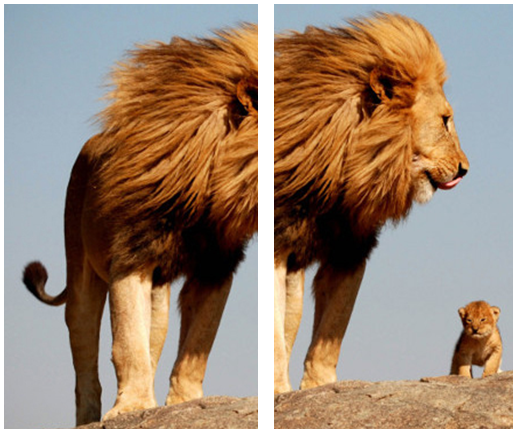
\includegraphics[width=0.45\textwidth]{fig/3.png}
     \vspace{-1em}
    \begin{center}    
       \caption{\textcolor{gray}{\footnotesize \textit{To billeder er af samme motiv, hvor kameraet fanger scenen fra to forskellige vinkler. F og F' angiver to korresponderende punkter, hvor den stiplede linje rammer de to scener \cite{kim}.}}}
    \label{fig:1}
     \end{center}
     \vspace{-2.5em}
  \end{figure} \noindent
I figur \ref{fig:1} ses to billeder af samme scene, men hvor kameravinklen er forskudt. For at opnå en korrespondance imellem billederne, skal der detekteres nogle unikke punkter, som optræder i begge billeder. I billedet er der udvalgt to korresponderende punkter \textit{p} og \textit{p'}. Disse punkter skal beskrives af en deskriptor \textit{D} så hvert punkt får tilknyttet en deskriptor $D(p)$ og $D(p')$. Det ønskes, for to korresponderende punkter, at: $D(p)\approx D(p')$ - en god deskriptor vil tillade, at korresponderende punkter bliver matchet korrekt. Korrespondanceanalysen består af følgende trin:
\begin{enumerate}
\item{Feature Detektion}
\item{Feature Deskription}
\item{Feature Matching}
\end{enumerate}
\section{Detektor}\label{sec:detect}
Feature detektion er en metode indenfor billedbehandling, der determinere, for hvert punkt (x,y) i et billede, om dette punkt er et interessepunkt.  En Feature detektor '$Det$' er en funktion, der tager et billede som input, $I$ og returnere et subset af isolerede punkter, $p_i$ fra billedet, som er vurderet til at være interessante. 
$$ Det(I)=\lbrace p_1,p_2,...,p_n \rbrace$$
Der er mange forskellige definitioner af hvad et interessepunkt er og i sidste ende angiver applikationsdomænet, hvilke punkter, der lokaliseres bedst. Interessepunkter kan f.eks. være kanter eller linjer i landskabet, ved genkendelse af veje fra satellitbilleder. Uanset hvilke strukturer, der ledes efter skal en detektor besidde følgende egenskaber:
\begin{itemize}
\item{\emph{Repeterbar}: Moravec \cite{moravec} definere et godt interessepunkt som værende et punkt, der entydigt kan lokaliseres i billeder, taget fra forskellige vinkler af en scene. Repeterbarheden significere detektorens uafhængighed af forskellige betingelser i billedet, dvs. dens evne til at detektere ens punkter i billeder, udsat for forskellige ændringer. }
\item{\emph{Distinktive:}
De fundne interessepunker skal være unikke ift. intensitetsvariationen i det omkringliggende område. Dette muliggør en mere akkurat lokal lokalisering af punktet.}
\end{itemize}
Ovenstående egenskaber kan opnås ved at tage højde for de ændringer, der kan forekomme i billederne, og derved være invariante overfor disse. Ændringerne kan være geometriske. F.eks. rotation, skalering (se figur \ref{fig:skal}) eller affine transformationer. Det kan også være fotometriske ændringer i form af intensitetsskift i billederne forsaget af lysændringer.
\begin{figure}[H]
    \centering
    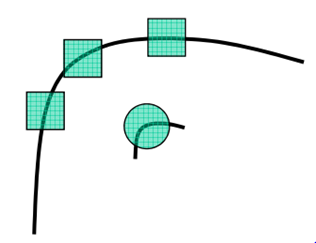
\includegraphics[width=0.37\textwidth]{fig/28.png}
     \vspace{-1em}
    \begin{center}    
       \caption{\textcolor{gray}{\footnotesize \textit{To ens kurver, der er set fra forskellige skalaer. Opfattes kurven langt væk fra, som den store kurve, vil de udvalgte områder opfattes som kanter. Skalere man ind på kurven vil området vise et hjørne. Det kan derfor, alt efter applikationsdomænet, være nødvendigt at anvende en skala invariant detektor.}}}
    \label{fig:skal}
     \end{center}
     \vspace{-2.5em}
  \end{figure} \noindent
Detektoren skal også være robust overfor små deformationer som støj i billedet, hvilket fejlagtigt kan fortolkes som interessepunkter. Interessepunkter defineres ikke udefra semantiske meningsfulde områder, som ansigter eller objekter, da dette vil kræve en høj-niveau fortolkning af scenen. I stedet anvendes lav-niveau strukturere, der identificeres i lokale pixel områder, som er matematisk definerbare og distinktive. Nedenstående er en gennemgang af forskellige lokale lav-niveau strukturere, der kan bruges i udvælgelsen af interessepunkter.
 \subsection{Hjørner}\label{subsec:corner}
En hjørnedetektor er en feature detektor, der definere et hjørne som værende et interessepunkt. Et hjørne kan defineres ved et punkt, der har to dominerende kanter i hver sin retning, derved er et hjørne et punkt, hvor der foregår store intensitetskift i det omrkingliggende område. Som følge af denne definition, er et hjørne distinktivt og kan bruges som interessepunkt. At detektere hjørner er en udbredt teknik indenfor feature detektion, hjørner ofte forekommer i forskellige menneskeskabte scener.
\begin{figure}[H]
    \centering
    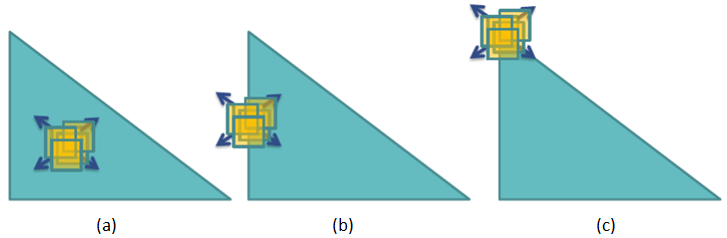
\includegraphics[width=0.55\textwidth]{fig/6.png}
    \vspace{-1em}   
    \begin{center}    
    \caption{\textcolor{gray}{\footnotesize \textit{
     Tre udvalgte vinduer, med interessepunkter i centrum af samme motiv. \textbf{(a)} Punktet er lokaliseret i en teksturløs region, d.v.s. ingen teksturskift. \textbf{(b)} Punktet er lokaliseret på en kant. \textbf{(c)} Punktet er lokaliseret på et hjørne }}}
    \label{fig:2}
     \end{center}
    \vspace{-2.7em}  
  \end{figure}  
\noindent
En intuitiv måde at definere hvorfor et hjørne er interessant, er at placere et rektangulært vindue omkring punktet. Dette vindue forskydes lokalt i x og y retningen. Opstår der et nyt objekt, identisk med interessepunktet, som resultat af forskydningen af vinduet er punktet ikke  distinktivt og derfor ej interessant. I figur \ref{fig:2} ses tre udvalgte punkter med et rektangulært vindue placeret over. I stil med ovenstående definition, forskydes det firkantede vindue i alle retninger. Forskydes \textbf{(a)} vil det ligne alle de forskudte billeder da punktet og regionen omkring punktet er homogent. Punktet er derfor ikke interessant. Forskydes \textbf{(b)} i x-aksen opnås et nyt objekt, men en forskydning i y-aksen vil resultere i samme objekt af en kant, og punktet er derfor ikke interessant. Punktet placeret på et hjørne \textbf{(c)} er interessant da ingen forskydninger vil ligne det originale billedet. Hjørnet kan derfor bruges som et interessepunkt. Denne intuitive definition kan kvantificeres til en matematisk definition, der estimere auto-korrelationen imellem de forskudte biller, hvilket angiver intensitetsskiftene imellem billederne og derved, hvor der opstår et hjørne. 
\subsection{Kanter}\label{subsec:kant}
Som nævnt er kanter ikke interessant, da de ikke er lokalt distinkte. Kanter kan dog bruges til at fjerne en del unødvendig information fra et billedet, ved kun at udtrykke kanterne.  En kant kan defineres ved at opfatte billedet som en funktion, der afbilder billedintensiteten i 1-dimension. En høj kurve, angiver et skarpt intensitetsskift og derved en kant. Kanter kan derved identificeres ved at finde disse skarpe sving i intensitetsfunktionen, se figur \ref{fig:kant}.
\noindent
\begin{figure}[H]
    \centering
    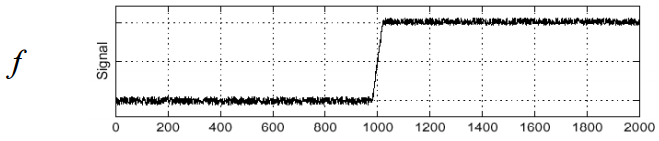
\includegraphics[width=0.55\textwidth]{fig/7.png}
     \vspace{-1em}
    \begin{center}        
     \caption{\textcolor{gray}{\footnotesize \textit{
     En 1-dimensional fortolkning af intensiteten i et billede. De små udsving indikere støj, den store kurve repræsenter et skrapt skift i intensiteten og derved en kant i et billedet.}}}
    \label{fig:kant}
     \end{center}
       \vspace{-2.5em}
  \end{figure}
\noindent
En differentiering af funktionen fra figur \ref{fig:kant} vil angive, hvor skarp kurven er og derved fremhæve dens udsving. Et 2-dimensionelt billede er ikke en kontinuerlig funktion, men består af diskrete værdier i form af pixel informationer.
Billedet differentieres derfor ved en approksimeret differentiering: \begin{equation}
\dfrac{df(x)}{dx}=\dfrac{f(x+1)-f(x-1)}{2}
\label{diff}
\end{equation}
\eqref{diff} kan udføres på billedet ved at folde billedet med kernen $[1 \hspace{0.5cm} 0 \hspace{0.5cm} -1]$. Foldning af et billede \emph{I} med indgangen $(M \times N)$, med en kerne \emph{K} med indgangen $(m \times n)$ , defineres ved operatoren: $I\ast K$ og udføres ved, for hvert punkt i billedet ved at udregne:
\begin{equation}
O(i,j) = \sum\limits_{k=1}^m \sum\limits_{l=1}^m I(i+k-1,l-1)K(k,l)
\end{equation}
Problemet ved differentiering, visualiseret i figur \ref{fig:kant}, er at støj i billedet (de små udsving) også vil blive fremhævet, hvilket kan resultere i fejlagtige detektioner af kanter. For at fjerne støjen foldes billedet med et Gaussisk filter, hvilket er en diskret approksimering til den Gaussiske funktion. Det Gaussiske filter beskriver et punkt, ved en vægtet normalfordeling af de omkringliggende pixelværdier. Foldning af et billede med et Gaussisk filter vil derfor resultere i en "flydende" overgang mellem pixel værdierne og derfor glatte billedet.  Den Gaussiske funktion i 2-D, hvor $ \sigma $ er standardafvigelsen af den Gaussiske fordelingen, er defineret som:
\begin{equation}
G(x,y,\sigma) = \frac{1}{2 \pi \sigma ^{2}} e^{- \frac{x^{2} + y^{2}}{2 \sigma ^{2}}}
\label{2dgaussian}
\end{equation} 
For at undgå itereration af billedet to gange, for differentiering og sløring, kan dette udføres i en samlet operation, ved at folde billedet med et differentieret Gaussisk filter, da foldning er en associativ operation.
\begin{equation}
\dfrac{\partial}{\partial x}(G \ast f) = (\dfrac{\partial}{\partial x}G) \ast f
\end{equation}
Udføres ovenstående på signalet fra figur \ref{fig:kant} vil det resultere i et "bakke" formet signal, hvor bakken indikere en kant. For en mere lokaliserbar kant, kan den dobbelt afledte bruges som set i figur \ref{fig:deriv}.
\begin{figure}[H]
    \centering
    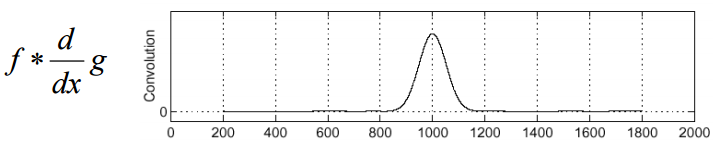
\includegraphics[width=0.55\textwidth]{fig/8.png}
    \vspace{-1em}   
    \begin{center}
    \caption{\textcolor{gray}{\footnotesize \textit{
     Resultatet af at folde et dobbelt differentieret Gaussisk filter med funktionen}}}
    \label{fig:deriv}
     \end{center}
    \vspace{-2.5em}  
  \end{figure}
\noindent
Kanten er nu let definerbar, ved at lokalisere når funktionen krydser nul. I et 2-dimensionelt billede repræsentere intensitetsskift også en orientering. Vertikale kanter findes ved at folde billedet med et Gaussisk filter, differentieret i x-aksen og y-aksen for horisontale kanter.
\subsection{Blobs}
En blob detektor finder regioner i billedet, der består af et sæt sammenhængnede pixels, alle af samme intensitet, der er distinktive ift. området. Lindenberg \cite{blob} definere blobs som værende lyse regioner på sort baggrund eller omvendt, altså strukturer, der står i kontrast til deres baggrund. En blob kan derfor defineres som et område med \emph{mindst} ét lokalt ekstrema, enten et maksima eller et minima.
\begin{figure}[H]
    \centering
    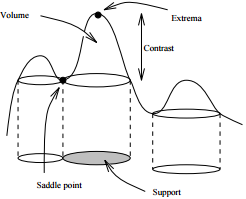
\includegraphics[width=0.35\textwidth]{fig/11.png}
    \vspace{-0.5em}   
    \begin{center}
    \caption{\textcolor{gray}{\footnotesize \textit{
    En blob visualiseret i 2-d, udefra Lindenberg's definition \cite{blob}}}}
    \label{fig:lindblob}
     \end{center}
  \end{figure}
       \vspace{-2.7em}
\noindent
I figur \ref{fig:lindblob}(a), ses en blob defineret af dets lokale ekstrema, hvor styrken af blobben beksrives ved kontrasten, ift. området omkring ekstremaet. Lindenberg definere blobbens domæne som værende afgrænset af dens "saddle point". Et "saddle point" angiver punktet, hvor intensiteten stopper med at falde og starter med at stige for lyse blobs, og modsat for mørke. Punktet definere altså blobbens domæne. Det lokale ekstrema gør blobben til en veldefineret lokal struktur og derved interessant. Blobs har også en fordel ift. kant og hjørne detektion, da blobs indgår i de fleste domæner. Kanter og hjørner forekommer ofte i menneskeskabte scener, ved veldefinerede strukturer. Blobs har derfor flere applikationsområder, og kan bruges indenfor billeder af objekter, der ikke er menneskelige defineret scener.  Ligesom i kant-detektion, kan blobs beskrives ved intensitetsskift, hvor der forekommer en krusning rundt om ekstremaet. En metode til at detektere disse ekstremaer hedder Laplace operatoren $\Delta^2$, defineret som:
\begin{equation}
\Delta^2 f = \dfrac{\partial^2 f}{\partial x^2}+\dfrac{\partial^2 f}{\partial y^2}
\end{equation}
 Laplace operatoren anvendes på et gaussisk filter og kaldes "Laplacian of Gaussian" eller "LoG" \eqref{lap}:
\begin{equation}
LoG=\sigma\Delta^2G
\label{lap}
\end{equation}
"LoG" operatoren kan diskritiseres og og foldes med billedet for at finde lokale ekstremaer. Figur \ref{fig:lapgauss} viser, hvordan laplace operatoren opnår et maximum i centeret af en blob, og at blobben derved bliver lokaliserbar. Hvis blobben (b), er tyndere eller tykkere vil laplace operatoren ikke længere resultere i et ekstrema, men nærmere en "bakke". Det er derfor nødvendigt at normalisere laplace filteret ift. hvilken størrelse blobben har.
\begin{figure}[H]
    \centering
    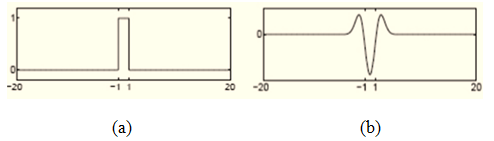
\includegraphics[width=0.60\textwidth]{fig/16.png}
    \vspace{-0.5em}   
    \begin{center}
    \caption{\textcolor{gray}{\footnotesize \textit{
    (a) En 3-D visualisering af en to-dimensional Laplacian of Guassian (b) ét en-dimensionalt signal (c) Laplacian of Gaussian operatoren anvendt på (b)}}}
    \label{fig:lapgauss}
     \end{center}
  \end{figure}
       \vspace{-2.5em}
\noindent
Blobs forekommer, ligesom andre strukturer, på forskellige skalaer, bestemt af størrelsen af objektet og objektets placering i billedet. I figur \ref{fig:scale} angiver cirklerne den undersøgte skala, hver skala illustrere forskellige objekter. Skala invarians er nødvendigt, hvis der forekommer ændringer i skalaen imellem billederne, men også for at detektere blobs af forskellige størrelser.
\begin{figure}[H]
    \centering
    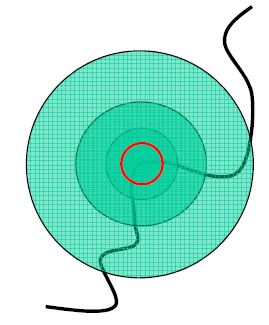
\includegraphics[width=0.25\textwidth]{fig/29.png}
    \vspace{-0.5em}   
    \begin{center}
    \caption{\textcolor{gray}{\footnotesize \textit{
    }}}
    \label{fig:scale}
     \end{center}
  \end{figure}
       \vspace{-2.5em}
\noindent
Så hvordan udvælges cirklen, der dækker interesse området uafhængigt af områdets størrelse?  For Blobs er det interessant når der i et skaleret område opstår et veldefineret ekstrema. En måde at søge efter ekstremaer over forskellige skalaer er ved at oprette et skalarum for det undersøgte billede, hvor hvert billede skaleres og der for hver skala udvælges features. Skala-rummet i et 2-dimensionalt billede repræsenteres af flere billeder i forskellige skalaer af det originale billede. Billeder, der repræsentere forskellige skalaer, opnås ved at folde billedet iterativt med et Gaussisk filter med stigende $\sigma$ værdi. 
\begin{figure}[H]
    \centering
    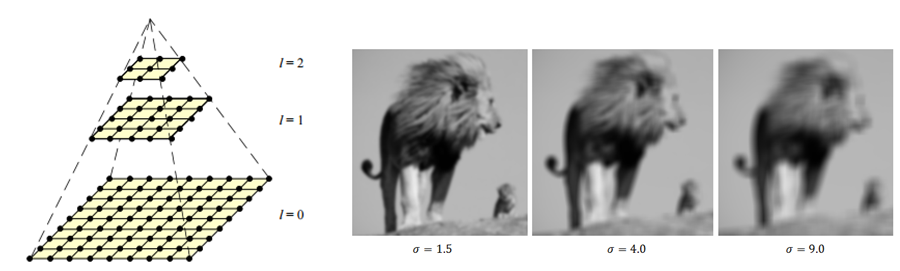
\includegraphics[width=0.65\textwidth]{fig/24.png}
    \vspace{-0.5em}   
    \begin{center}
    \caption{\textcolor{gray}{\footnotesize \textit{
Til venstre ses en visualisering af et skala-rum formet som en pyramide. Hvert niveau angiver en skala repræsentation af det originale vindue, hvor toppen af pyramiden indeholder billeder af største skala og derfor med mindst information, og bunden af skalaen med det originale billede. Til højre ses et billede foldet med et Gaussisk filter af stigende sigma værdier. Jo højere sigma værdi, jo flere fine detaljer bliver fjerne og billedet slørret.
    }}}
    \label{fig:mona}
     \end{center}
  \end{figure}
       \vspace{-2.5em}
\noindent
Et Gaussisk filter bruges da gradvis højere værdier af $\sigma$ fjerner fine strukturer, som vist i figur \ref{fig:mona} og nye strukturer forekommer ikke ved transformationen fra finere til grovere skalaer \cite{lindenscale}. Idéen er derved at fjerne disse strukturer og, lede efter  andre ekstremaer gradvist på større skalaer der også kan detekteres.
Et billede i skalarummet for billedet $f(x,y)$ kan derfor defineres som i \eqref{scalespace}
\begin{equation}
L(x,y,\sigma) = G(x,y,\sigma)\ast f(x,y)
\label{scalespace}
\end{equation}
hvor $G$ er det 2-dimensionelle Gaussiske filter,$L(x,y,\sigma)$ repræsentere et et billede i skala-rummet, og skala-parametren $\sigma$, bestemmer skalaen, eller placeringen i skala-rummet. $L(x,y,0) = f(x,y)$, da det er den "nederste" skala og den nederste del af pyramiden. Højere niveauer af pyramiden kan opnås ved at folde billedet med et Gaussisk filter af større sigma værdi.
\section{Deskriptor}
For at udvælge korresponderende punkter imellem billederne, skal interessepunkterne beskrives af en deskriptor $Des$. Deskriptoren er en funktion, der tager et billede og et punkt som input og returnerer en feature. Deskriptoren beskriver et interessepunkt ud fra information i og omkring punktet, og tilknytter punktet en feature $f$, i form af en n-dimensional vektor:
\begin{equation}
Des(I,p_i)=f_i
\end{equation}
\begin{equation}
Des(I',p_j')=f_j'
\end{equation}
For to korresponderende punkter $i$ og $j$ ønskes det at $f_i \approx f'_j$, så punkterne kan identificeres som værende korresponderende punkter, men også for to \textit{ikke} korresponderende punkter $k$ og $l$ at $f_k \not\approx f'_l$.
\section{Matching}
Fra deskriptoren er et sæt interessepunkter $p$ beskrevet ved features:
$$ Des(I,p)= \lbrace F_1,F_2,...,F_n \rbrace $$
$$ Des(I',p')=\lbrace F'_1,F'_2,...,F'_n \rbrace $$
Pga. ændringer i billederne vil korresponderende features aldrig være helt identiske, og der skal derfor oprettes nogle metoder, der kan determinere, hvornår 2 punkter er "ens" nok til at korrespondere.
Hver feature kommer i form af en x-dimensional vektor, der beskriver interessepunktet udefra noget data. Denne vektor skal sammenlignes med vektorer i det modsvarende billede, for at finde det bedste match. En metode er at undersøge den Euklidiske afstand mellem vektorene, hvor det "bedste match" kan kvantificeres til at være de vektor, der har de mindste Euklidiske afstande \eqref{euc}. 
\begin{equation}
||P|| = \sqrt{\sum\limits_{i=1}^n(q_i-p_i)^2}
\label{euc}
\end{equation}
Om to euklidiske afstande angiver et match kan defineres ved at sætte en sætte en grænseværdi. Der kan dog opstå visse problemer ved at sætte en sådan grænseværdi se figur \ref{fig:skift}. Forskellige transformationer i billedet kan også gøre at de målte afstande ligger længere væk end normalt eller omvendt, det er derved usikkert at definere en generel grænseværdi. En anden anvendelig metode er at matche med den "nærmeste nabo", hvor hvert punkt bliver matchet med den nærmeste euklidiske vektor. Her vil der også typisk sættes en grænseværdi for at fravælge dårligt defineret korrespondancer. Dette kan dog også være et problem i visse applikationer, hvor nogle punkter matcher flere punkter.
\begin{figure}[H]
    \centering
    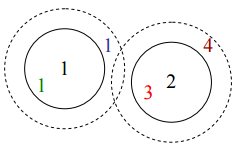
\includegraphics[width=0.35\textwidth]{fig/22.png}
    \vspace{-0.5em}   
    \begin{center}
    \caption{\textcolor{gray}{\footnotesize \textit{Problemet ved at sætte en grænseværdi: De sorte tal 1$\&$2 er features der skal matches mod et sæt andre features. Den solide inderste cirkel definere  en grænseværdi. Det grønne {\color{OliveGreen}1} er en sand positiv, det blå {\color{blue}1} er en falsk negativ(skulle havde været positiv), det røde {\color{red}3} er en falsk positiv (forkert vurderet). Sættes grænseværdien højere (til den stiplede linje) bliver det blå {\color{blue}1} en sand positiv, men den røde {\color{BrickRed} 4} bliver en falsk positiv. \cite{book1}}}}
    \label{fig:skift}
     \end{center}
  \end{figure}
       \vspace{-2.5em}
\noindent
Yderligere kan den "nærmeste-nabo" \textit{NN}\footnote{Nearest Neighbor}metode udvides til at kigge på den næst-nærmeste-nabo \textit{NNDR}\footnote{Nearest Neighbour Distance Ratio} ift. den "nærmeste-nabo", en metode introduceret i \cite{eval}.
\begin{equation}
N\!N\!D\!R=\dfrac{d_1}{d_2}=\dfrac{||D_A-D_B||}{||D_A-D_C|}
\label{nndr}
\end{equation}
hvor $d_1$ er den nærmeste-nabo distance og $d_2$ er den næst-nærmeste-nabo distance, $D_A$ er den udvalgte deskriptor, $D_B$ og $D_C$ er de to nærmeste naboer. Fordelen ved at anvende \eqref{nndr} ift. nærmeste-nabo, er at den straffer matches, der har en tæt euklidisk afstand med den næst-nærmeste nabo. Dette er fordelagtigt i visse sammenhæng f.eks. hvis man har nogle punkter, der matcher mange andre punkter, hvor man gerne vil have de distinktive matches, der kun har ét tydeligt korresponderende punkt se figur \ref{fig:skift2}.
\begin{figure}[H]
    \centering
    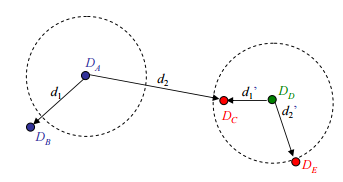
\includegraphics[width=0.35\textwidth]{fig/23.png}
    \vspace{-0.5em}   
    \begin{center}
    \caption{\textcolor{gray}{\footnotesize \textit{
      Matching med grænseværdi,\textit{NN} og \textit{NNDR} matching:
       Anvendes en simpel grænseværdi (stiplede linjer)  opstår der en falsk negativ med $D_A$ og $D_B$, $D_D$ matcher ukorrekt med $D_C$ og $D_E$    
       Anvendes metoden NN matcher $D_A$ korrekt $ D_B$, men matcher ukorrekt $D_D$ og $D_C$. Anvendes NNDR metoden matcher $D_A$ korrekt med $D_B$ og korrekt afviser match med $D_D$
     \cite{book1}}}}
    \label{fig:skift2}
     \end{center}
  \end{figure}
       \vspace{-2.5em}
\noindent